\hypertarget{performancetests_8cpp}{}\section{Gluonic\+L\+Q\+C\+D/tests/performancetests.cpp File Reference}
\label{performancetests_8cpp}\index{GluonicLQCD/tests/performancetests.cpp@{GluonicLQCD/tests/performancetests.cpp}}
{\ttfamily \#include \char`\"{}performancetests.\+h\char`\"{}}\newline
{\ttfamily \#include $<$chrono$>$}\newline
{\ttfamily \#include \char`\"{}config/parameters.\+h\char`\"{}}\newline
{\ttfamily \#include \char`\"{}parallelization/communicator.\+h\char`\"{}}\newline
{\ttfamily \#include $<$fstream$>$}\newline
{\ttfamily \#include $<$iomanip$>$}\newline
{\ttfamily \#include \char`\"{}math/exponentiation/expluscher.\+h\char`\"{}}\newline
{\ttfamily \#include \char`\"{}math/exponentiation/su3exp.\+h\char`\"{}}\newline
{\ttfamily \#include \char`\"{}math/exponentiation/taylor2exp.\+h\char`\"{}}\newline
{\ttfamily \#include \char`\"{}math/exponentiation/taylor4exp.\+h\char`\"{}}\newline
{\ttfamily \#include \char`\"{}math/exponentiation/taylorexp.\+h\char`\"{}}\newline
{\ttfamily \#include \char`\"{}actions/wilsongaugeaction.\+h\char`\"{}}\newline
{\ttfamily \#include \char`\"{}actions/luscheraction.\+h\char`\"{}}\newline
Include dependency graph for performancetests.\+cpp\+:\nopagebreak
\begin{figure}[H]
\begin{center}
\leavevmode
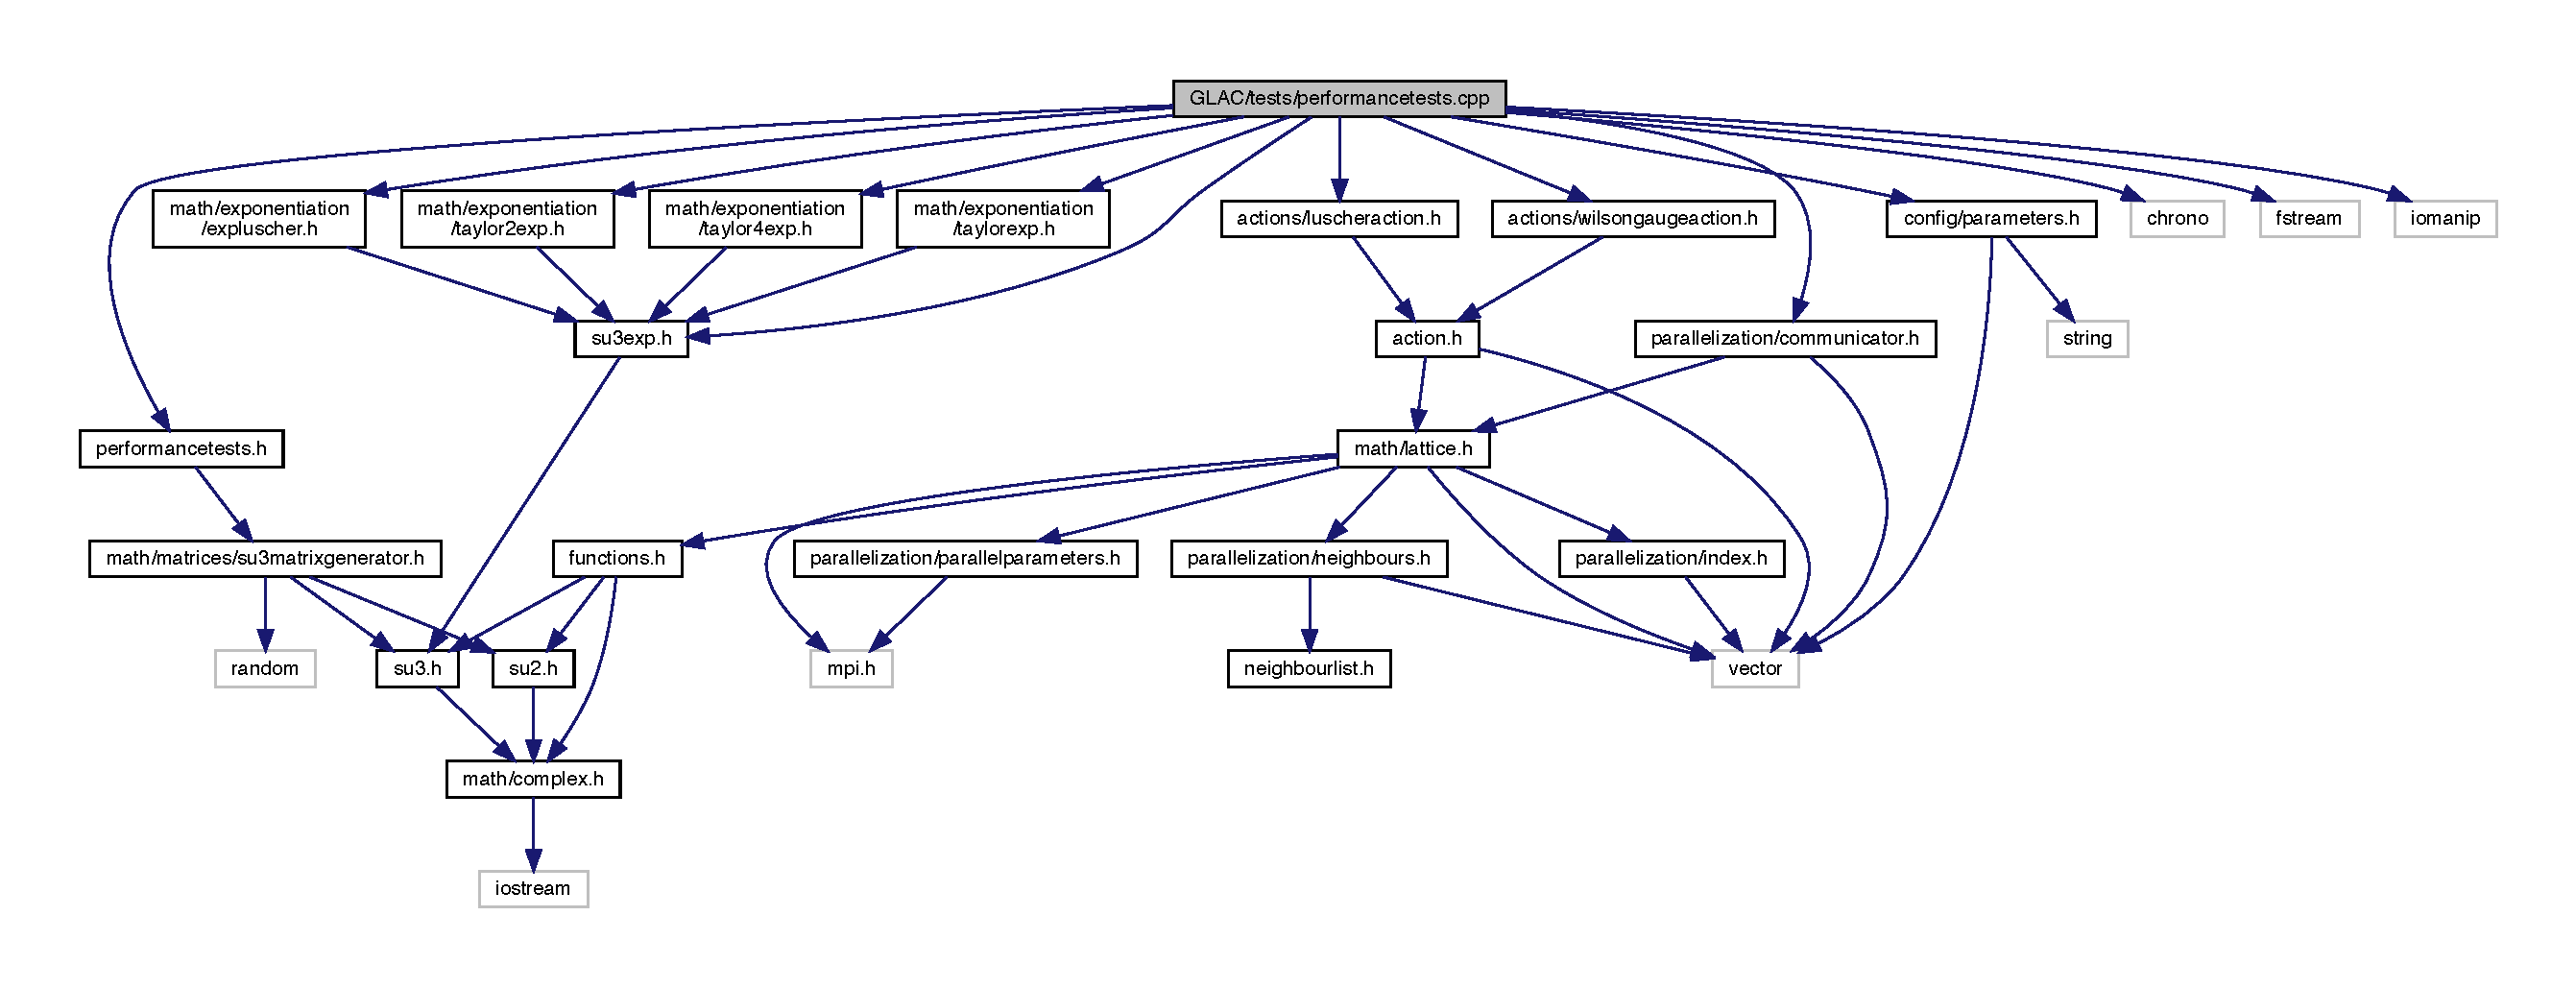
\includegraphics[width=350pt]{performancetests_8cpp__incl}
\end{center}
\end{figure}
